% Presentation modes
\documentclass[10pt]{beamer}
% Use for handouts
%\documentclass[10pt,handout]{beamer}

\usepackage[english]{babel}
% Package for horizontal rulers in tables  (e.g. \toprule)
\usepackage{booktabs}
% Handle page counting with appendix
\usepackage{appendixnumberbeamer}
% Package for positioning text/figures with absolute coordinates
\usepackage[absolute,overlay]{textpos}
% Package for code listings
\usepackage{listings}
% Referenceds
\usepackage{biblatex}
% Specify bib file
\addbibresource{cibiv.bib} 

\usetheme[progressbar=frametitle, titleformat=smallcaps]{metropolis}

\makeatletter
% Width of separator line on title page
\setlength{\metropolis@titleseparator@linewidth}{0.4pt}
% Width of progress bar
\setlength{\metropolis@progressinheadfoot@linewidth}{1pt}
% Width of progress bar on section pages (not used here)
\setlength{\metropolis@progressonsectionpage@linewidth}{0.4pt}
\makeatother

% CIBIV colors
\definecolor{dark_blue_cibiv}{HTML}{193848}
\definecolor{red_cibiv}{HTML}{D61F35}
\definecolor{blue_grey_cibiv}{HTML}{56778C}
\definecolor{grey_cibiv}{HTML}{89969F}
\definecolor{light_blue_cibiv}{HTML}{CFE3F2}
\setbeamercolor{frametitle}{fg=white,bg=dark_blue_cibiv}
\setbeamercolor{progress bar}{ fg=red_cibiv, bg=grey_cibiv }
\setbeamercolor{background canvas}{bg=white}
\setbeamertemplate{itemize items}[default]

% Left and right margin
\setbeamersize{text margin left=1.5em,text margin right=1.5em}

% logo
\titlegraphic{\vspace*{7cm}\hspace*{7.5cm}~%
   
\includegraphics[width=4cm]{img/cibiv_logo}
}

\lstdefinestyle{BLACK}
{
    backgroundcolor=\color{black},
    basicstyle=\footnotesize\color{white}\ttfamily,
    breaklines=true,
    xleftmargin=15pt,xrightmargin=15pt,
    framexleftmargin=1pt,
    framexrightmargin=1pt,
    framextopmargin=1pt,
    framexbottommargin=1pt,
    frame=ltb, framerule=0pt
}

% Document inf
\title{Cibiv Beamer Template}
\subtitle{Informative subtitle}
\author{John/Jane Doe}
\institute[CIBIV]{Center for Integrative Bioinformatics Vienna}
\date{\today}

% Defines a custom footer
% \setbeamertemplate{frame footer}{My custom footer}

\begin{document}

\maketitle

\begin{frame}{Requirements}
	
	\begin{itemize}
		\item<1-> The theme works with pdflatex and standard font
		\item<2-> However, I would \alert{recommend} installing \textbf{FiraFont} (\url{http://mozilla.github.io/Fira/}) and using \texttt{LuaLatex} for compiling
	\end{itemize}
	
\end{frame}

\section{Defining sections gives you this}

\begin{frame}{Figures (with handout option)}
	
	\begin{figure}[c]
		\includegraphics<1|handout:0>[height=0.9\textheight]{img/cibiv_webpage}
		\includegraphics<2|handout:1>[height=0.9\textheight]{img/cibiv_webpage_2}
	\end{figure}

\end{frame}

\begin{frame}{Picture overlay (absolute position)}
		
	\begin{itemize}
		\item \textbf{Alignments}
			Statistics of sequence alignment (i.e. mcmcalgn). Recently we have extended this approach to reconstruct an alignment and a phylogenetic tree simultaneously.
		\item \textbf{Sequence evolution}
			To understand sequence evolution it is necessary to model the substitution process. We are working on models sequence that allow dependencies among sequence sites (Markov fields seem to be an appropriate tool). We are developing test statistics to select the "best" model, to detect groups of sequence that evolve differently form the rest of a gene family, say. ...	
	\end{itemize}

	\begin{textblock}{8}(4, 5)
		\begin{figure}
			\includegraphics<2->[width=\textwidth]{img/cibiv_logo}
		\end{figure}
	\end{textblock}
	
\end{frame}


\begin{frame}{Tables}

	\begin{table}
		\caption{Largest cities in the world}
		
		\begin{tabular}{lc}
			\toprule 
			\textbf{City} & \textbf{Population}\\
			\midrule
			Mexico City & 20,116,842\\
			Shanghai & 19,210,000\\
			Peking & 15,796,450\\
			Istanbul & 14,160,467\\
			\bottomrule
		\end{tabular}

	\end{table}	
	
\end{frame}

\begin{frame}{Sided by Side}

	\begin{columns}
		\column{.5\textwidth}
			\begin{figure}[c]
				\vspace{-1.5em}
				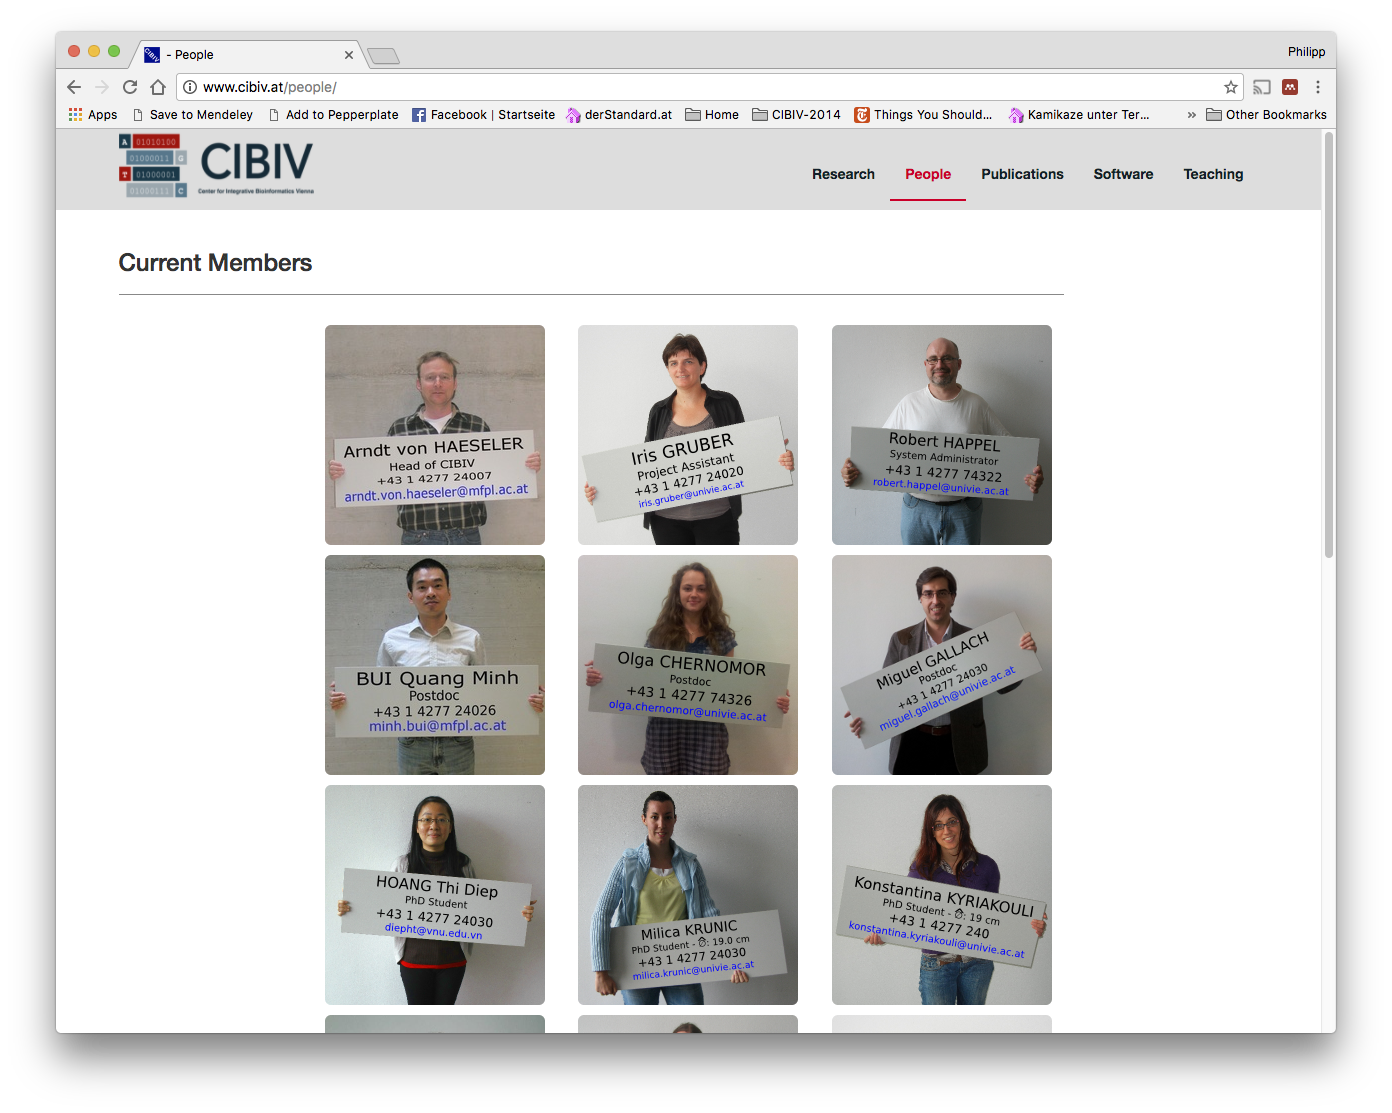
\includegraphics[width=1\textwidth]{img/cibiv_people}
			\end{figure}
		\column{.5\textwidth}
			\begin{itemize}
				\item Arndt
				\item Iris
				\item Robert
				\item Minh
				\item Olga
				\item Miguel
				\item ...
			\end{itemize}
	\end{columns}
	
\end{frame}

\begin{frame}{Blocks}
  Three different block environments are pre-defined and may be styled with an
  optional background color.

  \begin{columns}[T,onlytextwidth]
    \column{0.5\textwidth}
      \begin{block}{Default}
        Block content.
      \end{block}

      \begin{alertblock}{Alert}
        Block content.
      \end{alertblock}

      \begin{exampleblock}{Example}
        Block content.
      \end{exampleblock}

    \column{0.5\textwidth}

      \metroset{block=fill}

      \begin{block}{Default}
        Block content.
      \end{block}

      \begin{alertblock}{Alert}
        Block content.
      \end{alertblock}

      \begin{exampleblock}{Example}
        Block content.
      \end{exampleblock}

  \end{columns}
\end{frame}

% CAVEAT: lstlisting won't work without marking the frame as "fragile".
% If a frame is marked as "fragile" \begin{frame} and \end{frame} must NOT
% be indented
\begin{frame}[fragile]{Command line blocks / figure placeholder}

	\begin{lstlisting}[language=bash, style=BLACK]
$ tar cvf archive_name.tar dirname/
$ tar xvf archive_name.tar
$ tar -cjf - /directory/to/archive/ | wc -c
	\end{lstlisting}

	\begin{figure}
		\visible<2->{
\includegraphics[width=0.8\textwidth]{img/tar}}
	\end{figure}

\end{frame}


\begin{frame}{References}
	Here is text with a reference in the footer \footfullcite{Minh2013}\\
	Some references to showcase \cite{Nguyen2015}\\
	\fullcite{Minh2013}
\end{frame}

\appendix

\begin{frame}{Extra Slide}
	Not part of numbering	
\end{frame}

\begin{frame}[allowframebreaks]{References}

  \printbibliography

\end{frame}

\end{document}

